\subsection{User-side}
\label{sec:user-side}
% give an overview of the user-side system
% a web browser application
The front-end service of the system is a user serving web browser application accessible through the internet. 
The decision to use a browser application ensures that application is operating system-agnostic, which makes it available to more user devices. 
It also allows the system to remain up-to-date with any changes for all users, unlike native applications, which the user is responsible for updating. 
% The front-end application is used on desktop computers and standalone VR headsets. 
The instances of the application can be used on desktop computers, laptops, and standalone VR headsets, and communicate through a peer-to-peer connection, which allows them to coordinate with each other without routing data through a server. 
These web application instances serve as entry points to the embedded VR environment, which can be accessed through the VR headset. 
This is the environment where the user can see the visualised data, interact with the visualisation, manipulate it, and explore.

React.js is the framework chosen to implement the web application for VRDAVis, to replicate architectural choices from the CARTA system, as CARTA also uses React.js for its front-end application.
It is a free and open-source JavaScript library is used for building user-oriented applications based on components and can be employed to develop single-page, mobile, or server-rendered applications. 
It is maintained by Meta and a community of individual developers as well as companies.

In addition to React.js, MobX is a state management library designed for front-end web browser applications, responsible for maintaining stateful information. 
It integrates into React and is also used for state management within the CARTA framework.

% explain how the mipmap data supports functionality on the front-end
% no unneccessary rendering of points which equate to smaller than a pixel
% it returns a managable amount of data
% does not overwhelm the computer with the sheer amount of data it needs to process

% hosts some of the system logic
The front-end also hosts the majority of the system logic as it determines which piece or pieces of data need to be retrieved from the server. 
When the initial data is retrieved or the cube is cropped, a list of cubelets must be made so that the correct subsections can be fetched from the appropriate resolution level. 
The resolution level and lists are determined through a selection process taking into account the predetermined cubelet size, cubelets are selected from a mipmap level which maximises the resolution while maintaining performance. 
It is biased towards the mipmap layer with the maximum downsample ratio, which reduces the total number of cubelets that cover a selected area, whether it is the whole cube or a subset of the cube. 
This strategy limits the maximum amount of data that can be sent to the client. 

This selection process is critical when the cube is cropped on the front-end, as it discards portions of the cube that are not being focused on. 
Figure \ref{fig:crop-cube} illustrates the relationship between the cropped portion of the cube and the cube space, showing the dimensions of the full-resolution cube, as well as how multiple cropping actions relate to each other. 
Each crop action selects a subset of the previous cube.

The algorithm used to crop the cube and select cubelets at a higher resolution level can be broken down into the several steps:
\begin{enumerate}
    \item To determine which cubelets need to be requested initially, the full-sized data cube is cropped with a selection boundary of the same size.  The cube localspace is the current state of the cube being visualised on the front-end application, and the crop cube is the subset of the cube for which higher resolution cubelets are going to be requested.
    \item Every time the cube is cropped, the visualised cube's space and crop cube's space are aligned in the full-resolution cube's space, which can also be referred to as the cube's worldspace, encapsulating the full resolution dimensions. This is done to ensure that the crop cube's corner coordinates fall within the x, y, and z dimensions of the cube's coordinates. This is achieved through the multiplication of the crop cube dimensions and the centre coordinates by the current mipmap level. The initial mipmap level for the XY and Z axes is set to 1, and when the cube is cropped, the cube localspace dimensions and centre are updated to equal the crop cube's dimension and centre.
    \item The corners are calculated by the division of the dimensions by 2 then the addition or subtraction of this number to the centre for the x, y, and z dimensions.
    \item The crop cube's dimensions and centre are translated to coordinates within the full-resolution cube.
    \item The maximum mipmap level that data can be fetched from is determined by the adjustment of the crop cube corners to coordinates within the data cube, so that the centre of the axis shifts from zero to the midpoint of the full-resolution cube dimensions. This point is referred to as the adjusted centre.
    \item The current mipmap for XY and Z is initially set to 1. The minimum and maximum values of x, y, and z dimensions are determined to establish which cubelets are fully or partially inside the cropped area.
    \item The crop cube dimensions are rounded to the nearest cubelet boundary. 
    \item The process then steps through each range from the minimum boundary to the maximum boundary level. 
    \item The step is divided by the cubelet dimension size to determine the encoded coordinate of the cubelet needed from the data server.
\end{enumerate}
% mipX = Math.pow(2, Math.ceil(Math.log2(this.cropCube.x * this.currentXYMip)))/CUBELET_SIZE_XY;
% mipZ = Math.pow(2, Math.ceil(Math.log2(this.cropCube.z)))/CUBELET_SIZE_Z;
% Where the begining and end of each dimension of the cube in mipmap level is determined by
% const xStart = Math.floor((cubeState.xMin / cubeState.mipXY) / CUBELET_SIZE_XY) * CUBELET_SIZE_XY;
% const xEnd = Math.ceil((cubeState.xMax / cubeState.mipXY) / CUBELET_SIZE_XY) * CUBELET_SIZE_XY;
% \[ maxmip_x = 2^\frac{\cdot{cropCube_x}{currentMip_x}}{cubelet_x} \]

\begin{figure*}
    \centering
    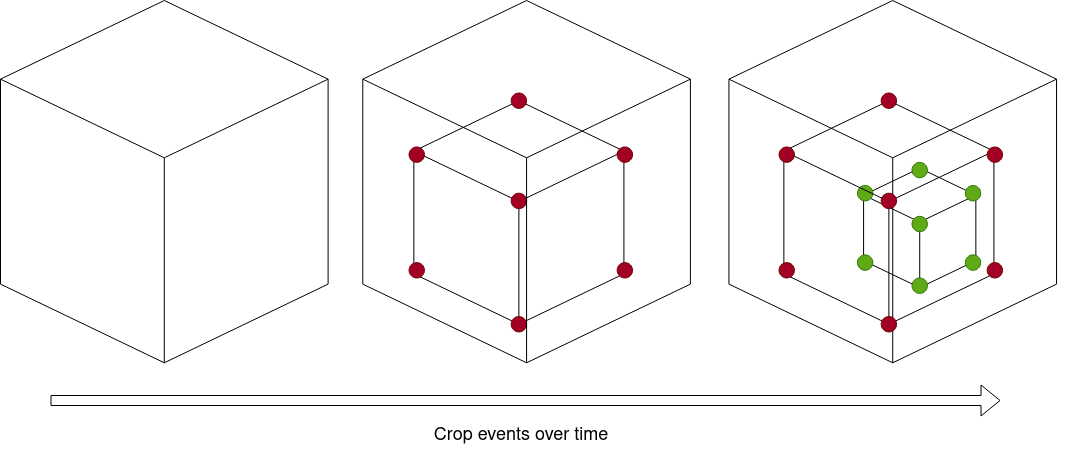
\includegraphics[width=0.6\linewidth]{figures/crop-cube.png}
    \caption{The relationship of the crop cube across cropping events to the full resolution data cube as the user drills down into a section of interest. The cropped sections refer to the marked red and green squares in the diagram; these sections are a selection made during a crop action. They are the portion of the data used to create the visualisation in the front-end services.}
    \label{fig:crop-cube}
\end{figure*}

% Virtual Reality Environment
% As the popularity of VR has boomed in recent times, there have been major developments in VR technology, driven by the demand for VR devices in the entertainment industry ~\cite{Farr2009}. 
% The virtual reality component of the front-end is embedded in the web browser application, and with packages like Three.js and WebXR, VR and three-dimensional environments can be embedded into web pages. 
WebXR grants access to the display of the headset, as well as the positions of the camera and controllers, allowing for integration with the web. 
Three.js was used to create the assets within the VR environment, such as the data cube used to display the astronomy data, and the UI elements which use canvases as textures to display text on a plane. 
These elements are made interactive through WebXR functions. 
The combination of these libraries facilitates a VR experience through the internet.
The data visualisation is presented within the VR space as a cube mesh with a three-dimensional texture used to map the three-dimensional data. 
This presentation method was selected because of its minimal processing cost~\cite{Ferrand2018}.
% choice to use volume rendering
%   present the data as is with minimal processing
%   iso-surface models must be generated using the raw data

% performs the rendering of the data
The data visualised by VRDAVis is volumetric astronomy data; however, this system would be able to visualise any volumetric data as long as it is in the HDF5 file format.
The HDF5 schema used is the same schema used by the fits2idia repository~\cite{fits2idia}, which is used to convert FITS files into the HDF5 files.
The mipmaps in the HDF5 file are stored according to their downsampling ratios.
For example XY\_2\_Z\_4 means that the x and y axis have been downsampled to a size 2 times smaller than the original cube and the z axis has been downsampled 4 times smaller than the original cube. 
The data arrives at the front-end from the data server in a float array format, where it is placed in a three-dimensional texture and rendered using a ray-cast shading technique.
The process of the ray-casting shader has the following steps:
\begin{enumerate}
  \item A ray is cast until it hits a bounding box of the volume texture.
  \item The ray takes a step through the volume and samples a point from the three-dimensional texture.
  \item The values that the ray sampled are added to an accumulator to determine the opacity of the pixel.
  \item The shader keeps track of the maximum value the ray has sampled.
  \item The ray continues to sample points until it has reached its maximum step count or the accumulated opacity reaches a 100\%.
  \item The shader then samples a two-dimensional colour map texture to retrieve a colour value for the pixel.
  \item If the opacity of the pixel is 0\%, the point is discarded.
\end{enumerate}

The rendering of the data with a ray-casting shader was implemented with the Three.js framework~\cite{Danchilla2012}, it can be easily integrated with React.js, a cross-browser JavaScript library built on top of WebGL. 
It is used to create and animate three-dimensional computer three-dimensional graphics within web browsers.
Three.js is widely adopted, and benefits from an active community that offers robust support. 

The shader goes through these steps for every frame, for every pixel on the screen. % cite
This is the most computationally expensive step in the visualisation process. 
Although ray-cast shading is computationally expensive, it depicts the data in a way that closely matches its structure, as if it were a high-resolution three-dimensional scatter plot.

For the user to view the visualisation with the VR headset in a virtual environment, a package is require which makes the three-dimensional environment compatible with VR displays and controllers.
WebXR provides access to input data related to the pose information from the headset and controllers, and output, which is the display within the headset. 
This technology enables web browsers to facilitate Virtual Reality (VR) and Augmented Reality (AR) experiences over the internet. 
It encompasses functionalities commonly associated with VR and AR devices.

In VRDAVis, WebXR is used to integrate an embedded VR environment into the client web application. It works in conjunction with Three.js and React.js to create an immersive three-dimensional environment, constituting the VRDAVis front-end application.

\subsubsection{User Workflow}

\begin{figure*}
    \centering
    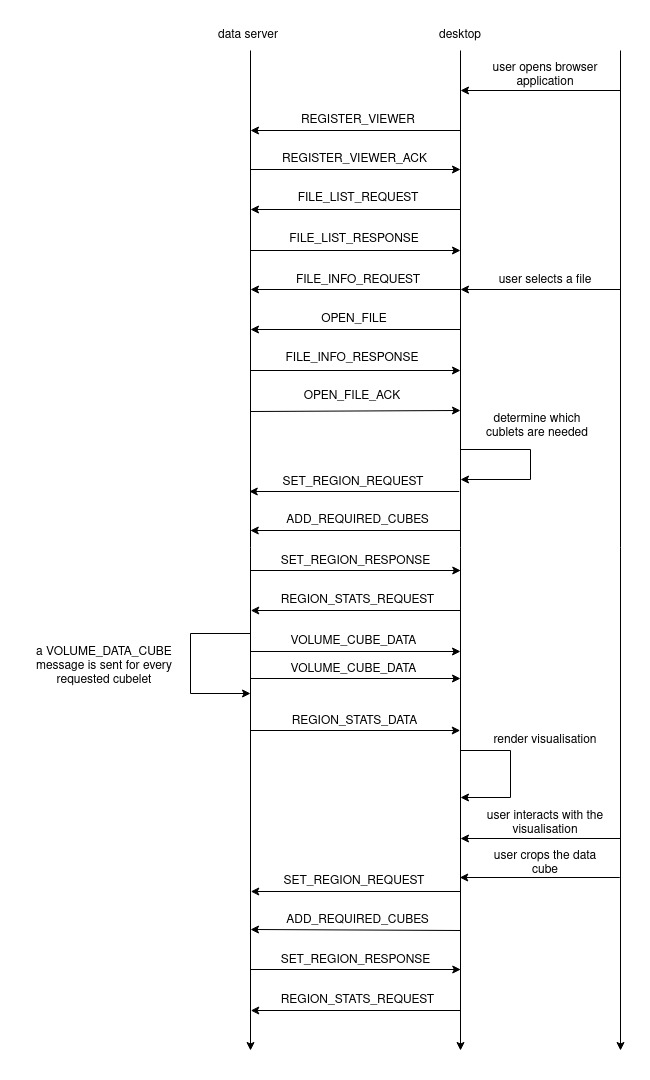
\includegraphics[width=0.6\linewidth]{figures/user-worklow(4).jpg}
    \caption{ A sequence diagram showing the user's interaction with an instance of the client application and the corresponding protocol buffer messages which are sent from the front-end to the back-end, as well as the responses from the back-end to the front-end. It shows the message sequence of the user opening the front-end application, selecting a file from a list, and cropping the visualisation.
    }
    \label{fig:user-workflow}
\end{figure*}

The user first opens an instance of the browser application on their desktop computer. 
When it is launched, this application instance creates a connection with the remote services such as the data and signalling servers. 
The signalling server connects the desktop client instance and pairs with the standalone VR headset if it is also connected to the signalling server at that time. 
This connection is made automatically once both devices are connected to the server. 
If the desktop device is not paired, then the user can pair it with an available unpaired device. 
When this peer-to-peer connection is created, the state of the visualisation can be transferred between the paired devices. 
The data server acknowledges the client application's connection, and the client requests a list of the available files on the server.

\begin{figure}
    \centering
    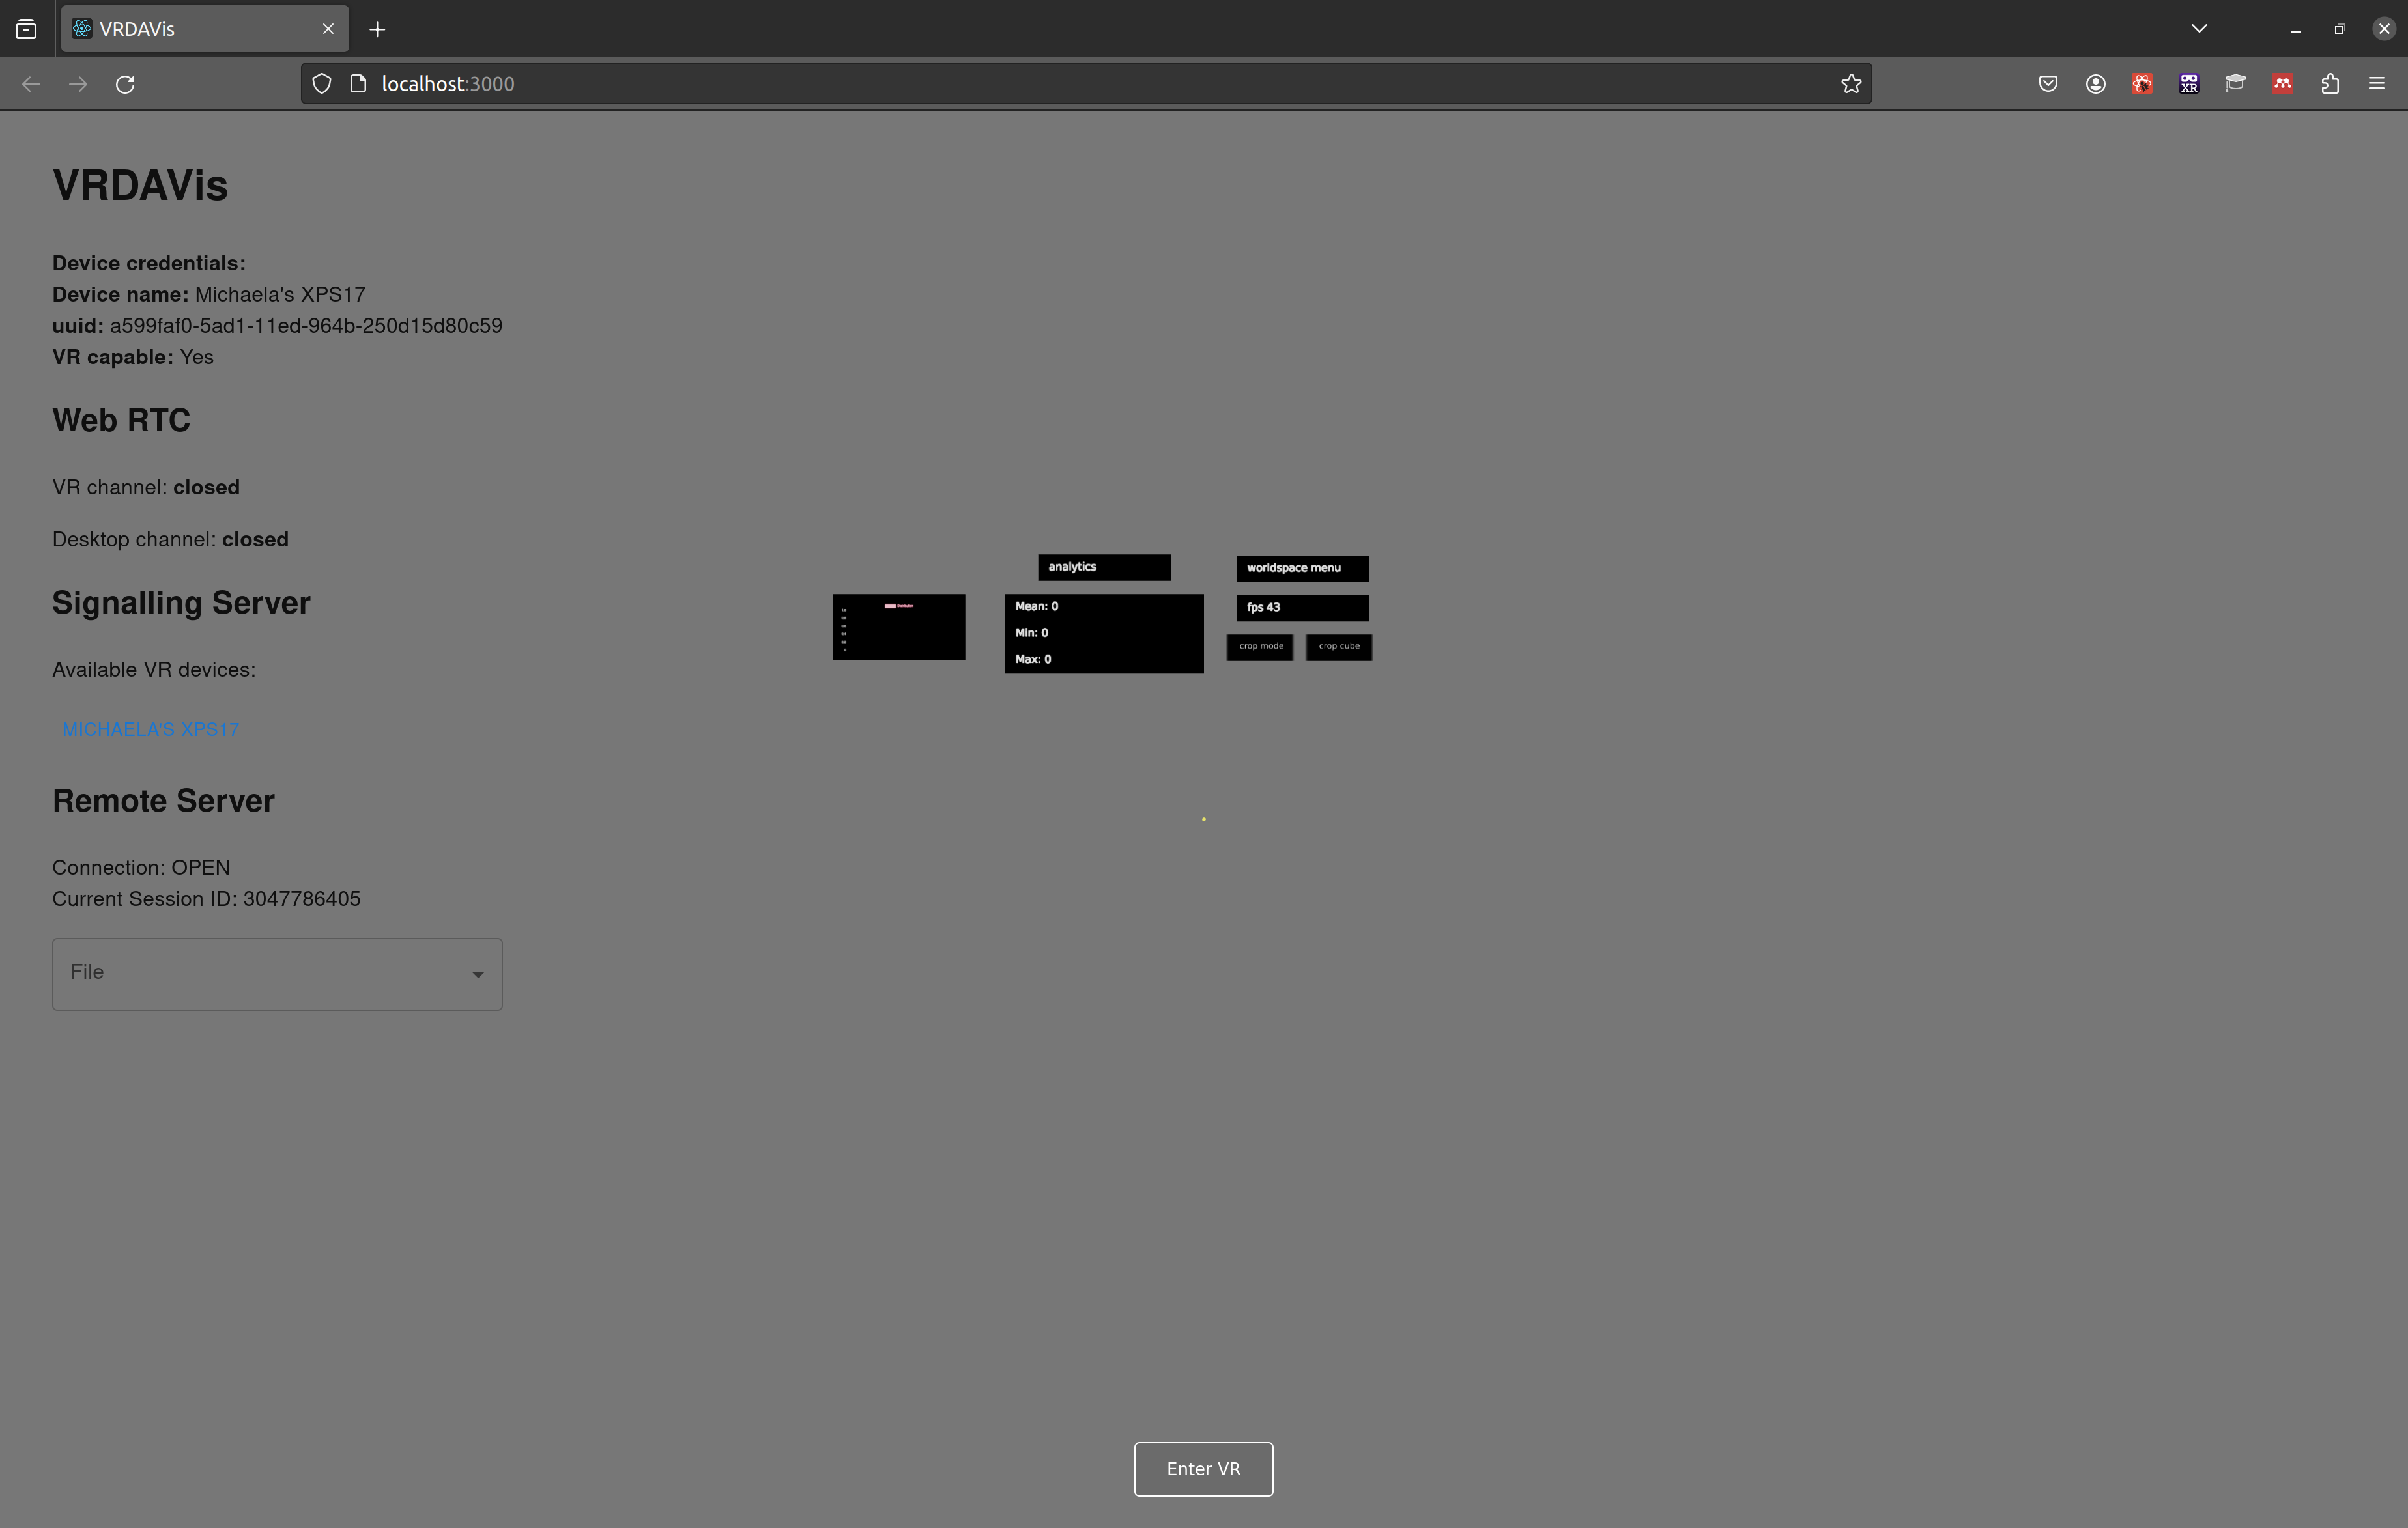
\includegraphics[width=\linewidth]{figures/screenshots/1.png}
    \caption{The appearance of the VRDAVis application when it is fist opened in the browser. In this instance the browser is Firefox. Some information about the current session can be seen on the left side of the screen, as well as the status of the peer-to-peer connection under the Web RTC heading, the available VR devices which can be paired with under the Signalling Server heading, and a drop down menu for selecting a data cubes under the Remote Server heading. Some VR environment assets can be seen in the centre of the screen.}
    \label{fig:screenshot-1}
\end{figure}

\begin{figure}
    \centering
    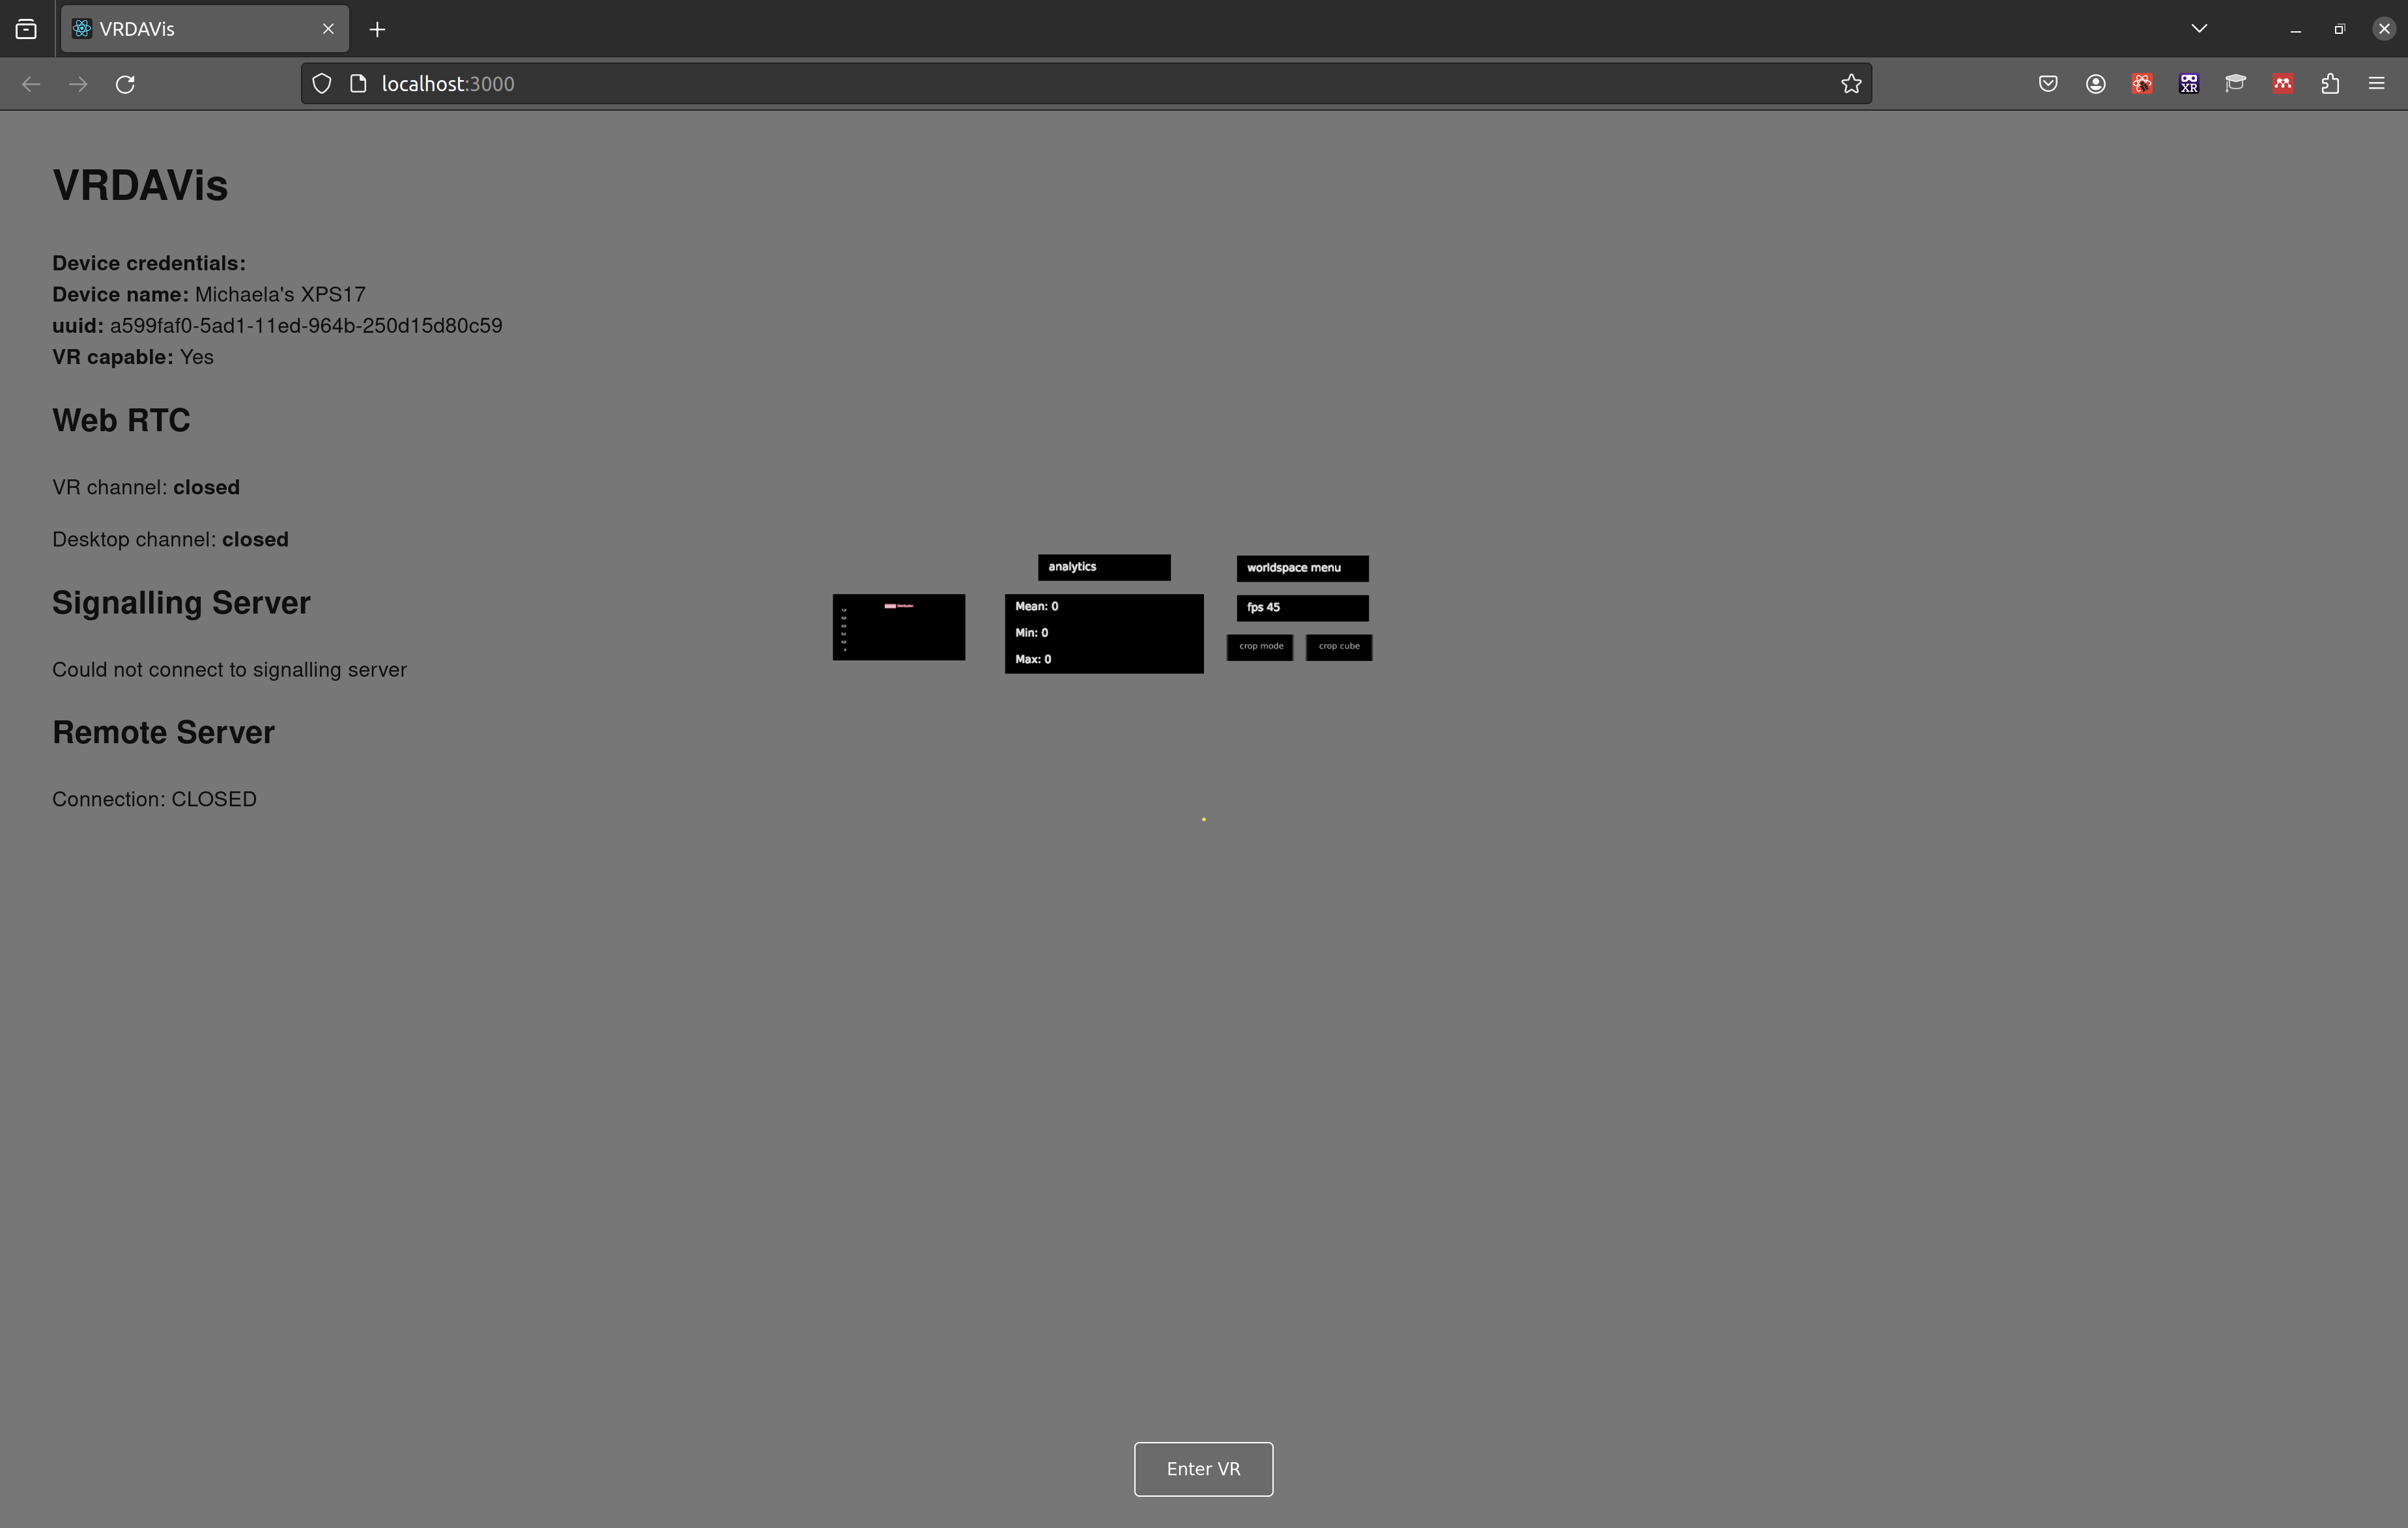
\includegraphics[width=\linewidth]{figures/screenshots/4.png}
    \caption{The appearance of the browser application when none of the remote services are available; there is no peer-to-peer connection, no connection to the signalling server, and no connection to the remote server.}
    \label{fig:screenshot-4}
\end{figure}

The data server sends the file list, and the user can choose which file they would like to explore. 
The user's file choice is sent to the data server, and the data server sends back some information pertaining to the selected file, such as dimensions and the size of the file. 
The client determines which cubelets it requires to generate the initial visualisation and requests them from the data server, while also specifying which analytics the data server needs to compute using the full-resolution data. 
The data server opens the file, reads the cubelets the client requested, compresses these cubelets into individual messages, and sends them to the client. 
Once the analytics are computed, they are also sent to the client.

When a cubelet reaches the client, it is decompressed and loaded into the GPU cache. 
The cubelet is then added to the three-dimensional, one at a time, until all the cubelets have been received and added. 
This three-dimensional texture is then rendered by the ray-casting shader.

\begin{figure}
    \centering
    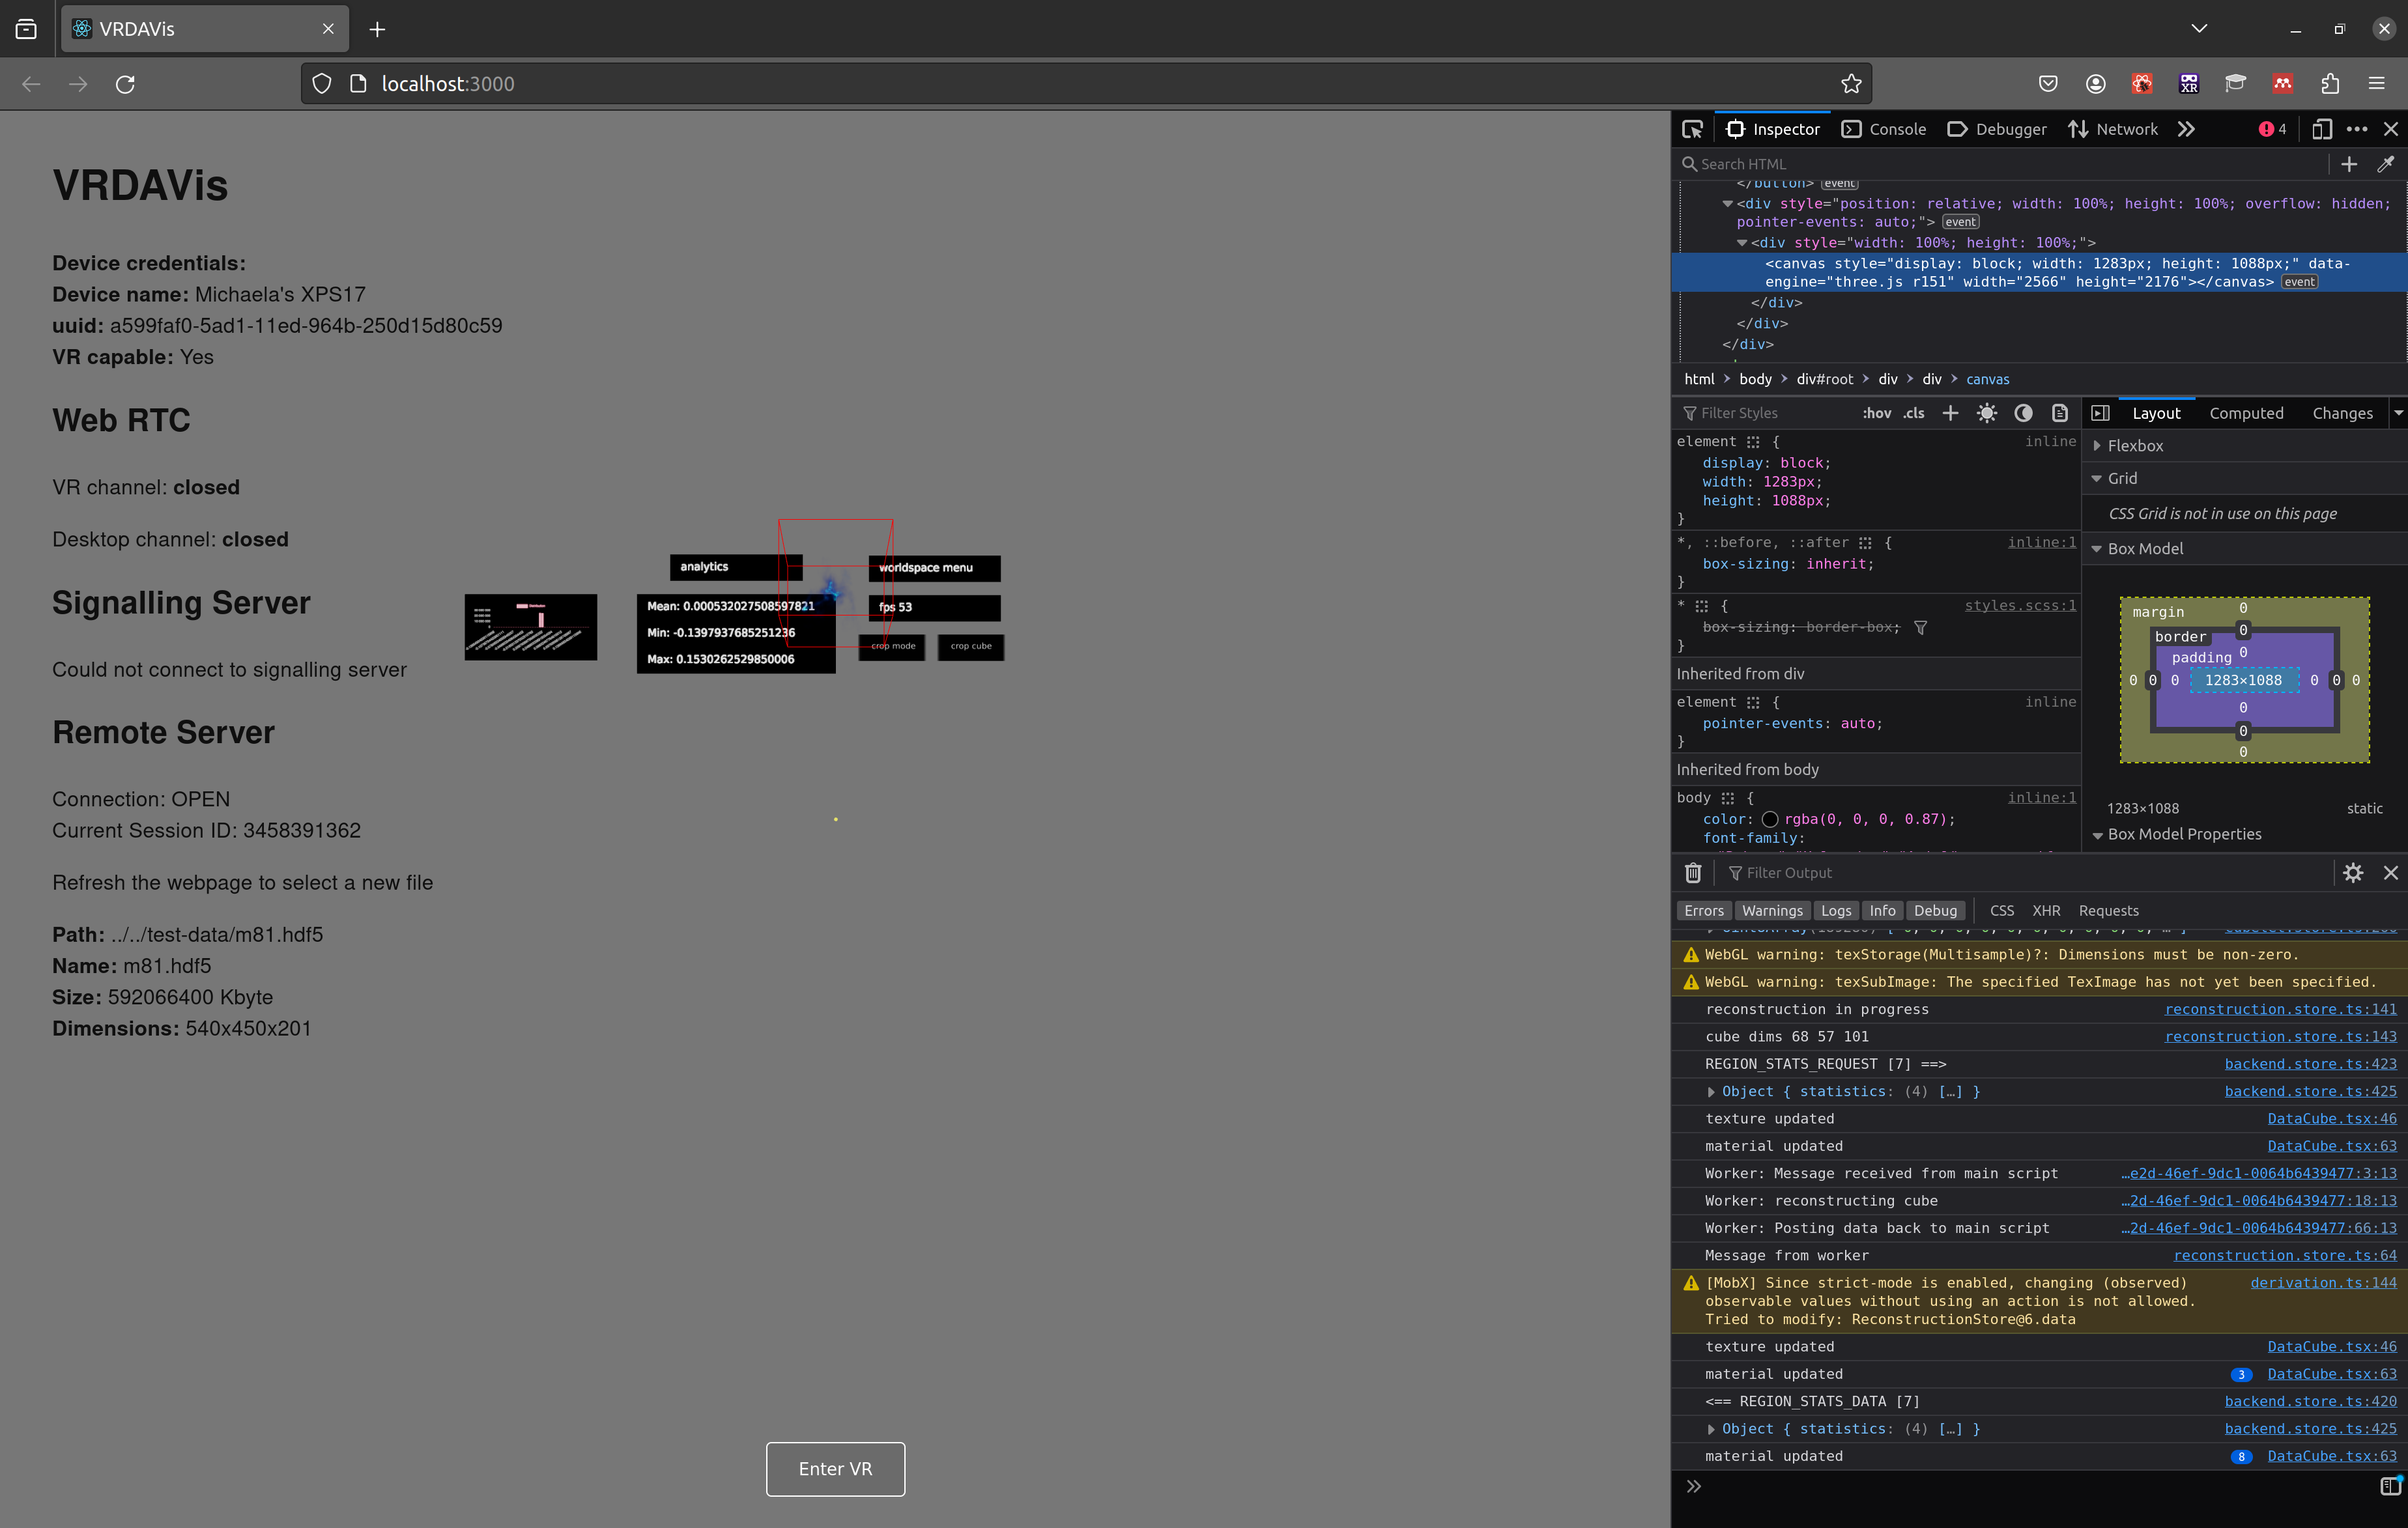
\includegraphics[width=\linewidth]{figures/screenshots/5.png}
    \caption{The view of the web browser application when a file has been selected and an initial visualisation of the data cube is within the VR environment. Some additional information about the data cube is displayed under the Remote Server heading; the path of the file on the remote server, the name of the file, the size in kilobytes, and the dimensions of the data cube.}
    \label{fig:screenshot-5}
\end{figure}

The user can then choose to switch to viewing the visualisation on the standalone VR headset. 
If the user switches to the headset, all the state information is sent over the peer-to-peer connection. 

The headset client uses the state information to start its own session on the data server and request the same cubelets as on the desktop client instance. 
The VR instance does not need the desktop instance to function; the user can choose to start the entire visualisation process on the VR headset by starting the client browser application on the browser. 
The main difference between the instance of the application on the desktop and the VR headset is that the VR headset client instance has the entry point to the VR environment, whereas the desktop does not have the capabilities to view a VR environment.

When the user enters the VR environment, they can interact with the visualisation in a three-dimensional space and view the analytics of the data. 
\begin{figure}
    \centering
    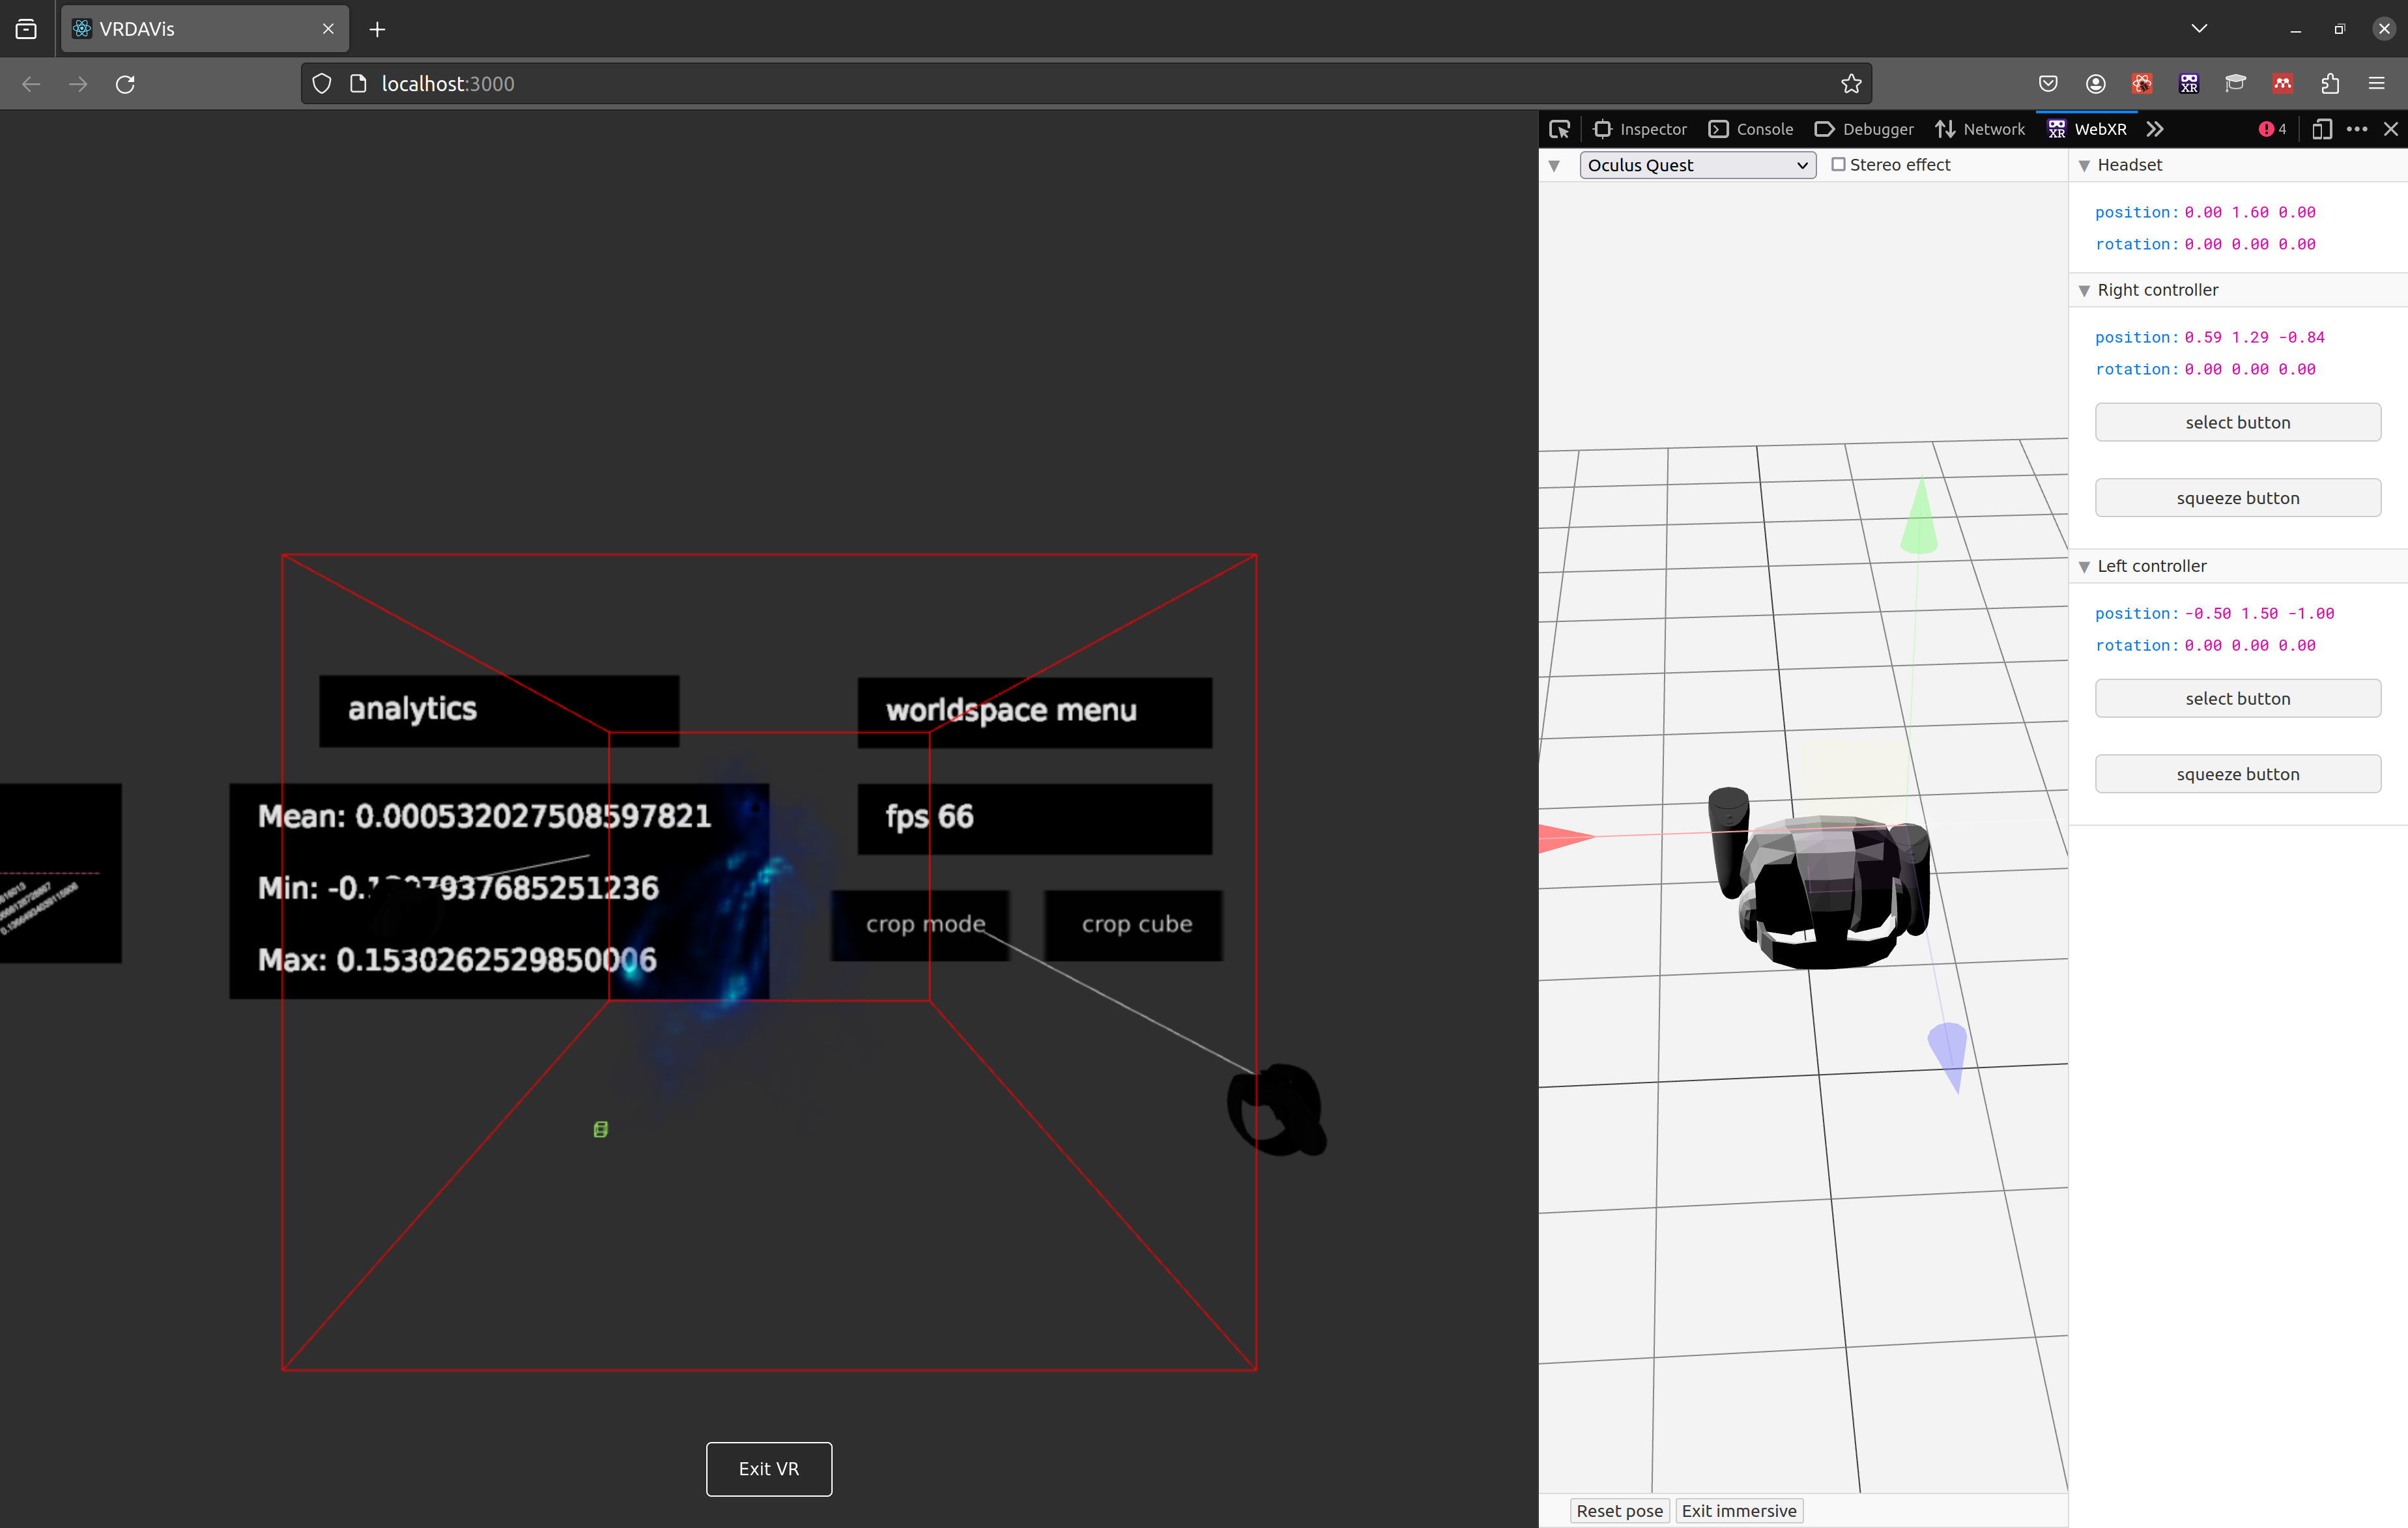
\includegraphics[width=\linewidth]{figures/screenshots/9.png}
    \caption{The view from inside the VR environment. The assets which could be seen on the centre of the view are now tangible within the VR environment. The data-cube is now a three-dimensional object and the analytics menu can be seen behind it. The WebXR browser plugin is used to view the VR environment from the browser window on a conventional screen. The plugin interface is displayed on the right side of the browser window.}
    \label{fig:screenshot-9}
\end{figure}
The user can crop the visualisation to get a higher-resolution version of the data by using the crop function; the user drags a box over the section they would like to take a closer look at and then selects the crop button. 
The client application determines which resolution level is appropriate for cubelet selection and sends a list of cubelets to the data server. 
The server fetches the cubelets and computes the analytics in the same way as it did for the initial visualisation. 
This process happens every time the cube is cropped until it reaches the highest resolution level, which is the full-resolution data. 
The size of the cubelets is determined by predetermined, internal values in the remote and front-end services.

\begin{figure}
    \centering
    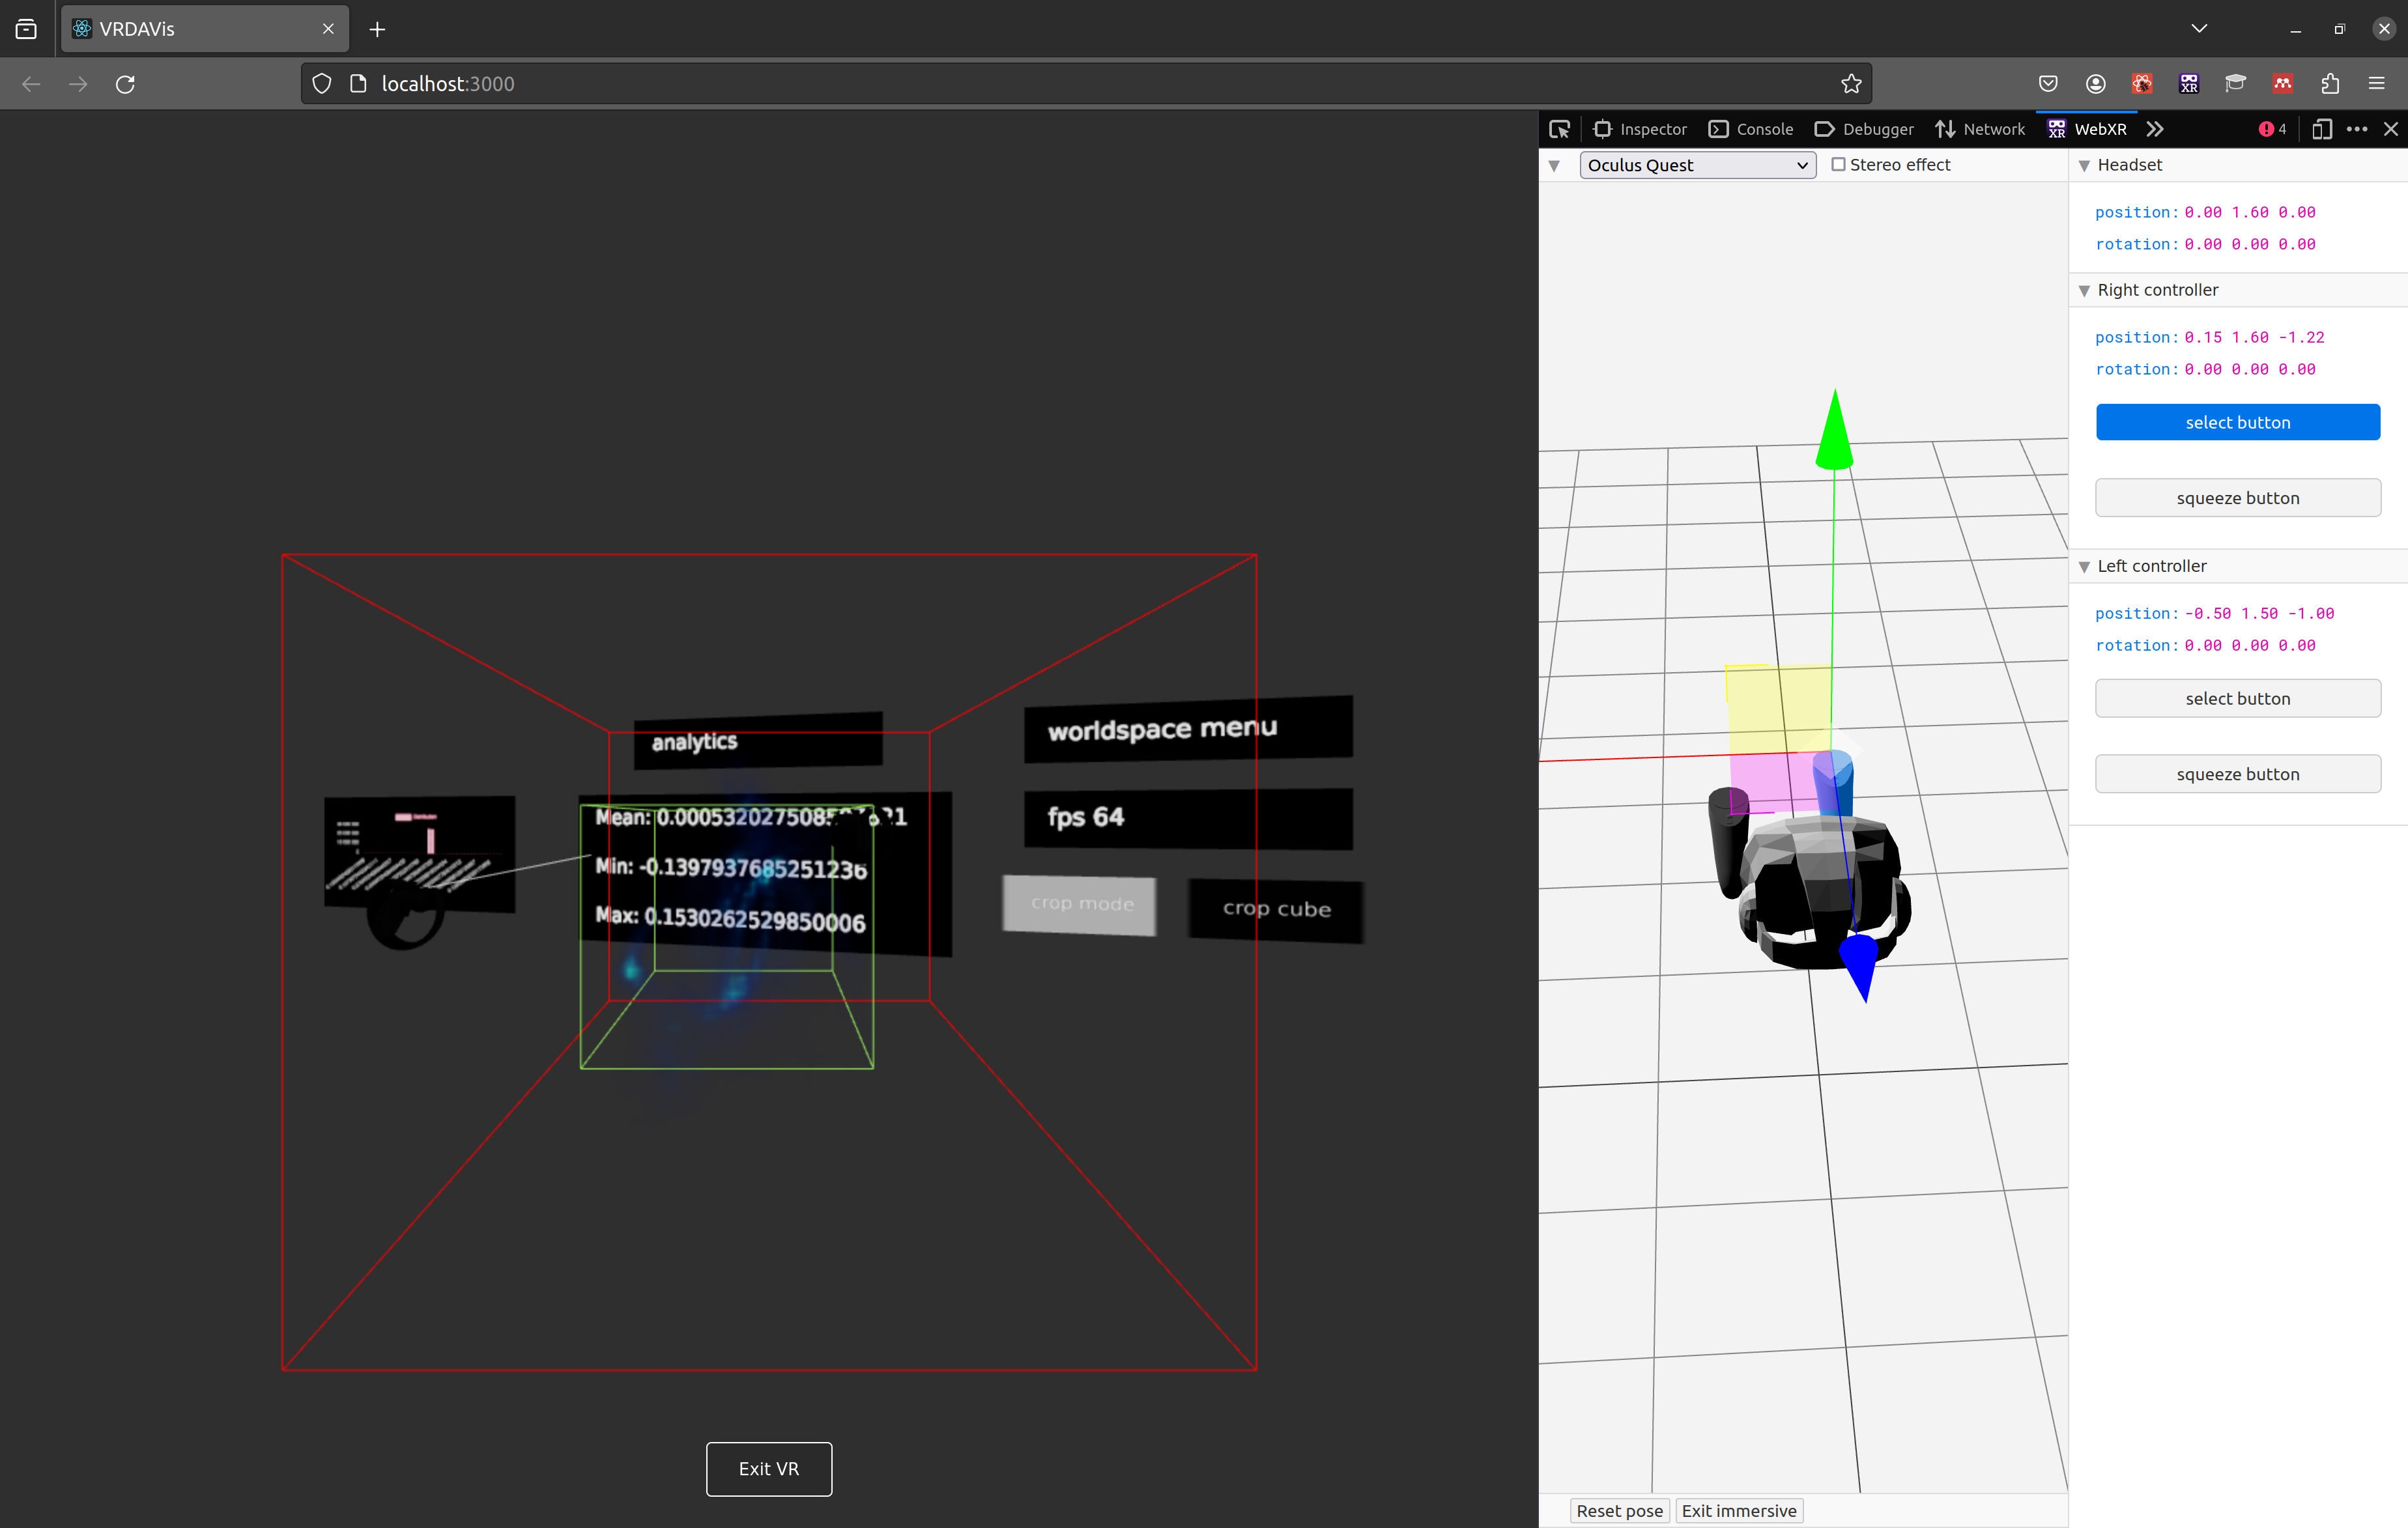
\includegraphics[width=\linewidth]{figures/screenshots/10.png}
    \caption{An example of a data cube displayed in the VR environment. The red cube represents an area within full dimensions of the data cube, and the green cube shows the selected crop area.}
    \label{fig:screenshot-10}
\end{figure}